\section{Adjusting the queuing model}\label{sec:scenarios}

This section is comprised of several `what-if' scenarios --- a classic component
of healthcare operational research --- under the novel parameterisation of the
queue established in Section~\ref{sec:model}. The outcomes of interest in this
work are server (resource) utilisation and system times as these metrics capture
the driving forces of cost and flow as well as the overall state of the system,
its staff and its patients. Specifically, the objective of these experiments is
to address the following questions:
\begin{itemize}
    \item How would the system be affected by a change in overall patient
        arrivals?
    \item How is the system affected by a change in resource availability (i.e.\
        a change in \(c\))?
    \item How is the system affected by patients moving between clusters?
\end{itemize}

Owing to the nature of the observed data, the queuing model parameterisation
and its assumptions, the effects on the chosen metrics in each scenario are
given in relative terms with respect to the base case. The base case being those
results generated from the best parameter set recorded in
Table~\ref{tab:comparison}. In particular, the data from each scenario is scaled
by the corresponding median value in the base case meaning that a metric having
a value of 1 is `normal'.

As mentioned in Section~\ref{sec:intro}, the source code used throughout this
work is available online and has been archived. %TODO Add citation for repo
In addition to this, the datasets generated from the simulations in this section
have been archived along with those generated from the parameter
sweep~\cite{Wilde2020results}.


\subsection{Changes to overall patient arrivals}\label{subsec:arrivals}

Changes in overall patient arrivals to a queue reflect real-world scenarios
where some stimulus is improving (or worsening) the condition of the patient
population. Examples of stimuli could include an aging population or
changes to deprivation. Within this model, overall patient arrivals are altered
using a scaling factor denoted by \(\sigma\in\mathbb{R}\). This scaling factor
is applied to the model by multiplying each cluster's arrival rate by
\(\sigma\). That is, for cluster \(i\), its new arrival rate, \(\hat\lambda_i\),
is given by:
\begin{equation}\label{eq:lambda}
    \hat\lambda_{i} = \sigma\lambda_i
\end{equation}

\begin{figure}
    \centering
    \begin{subfigure}{.5\imgwidth}
        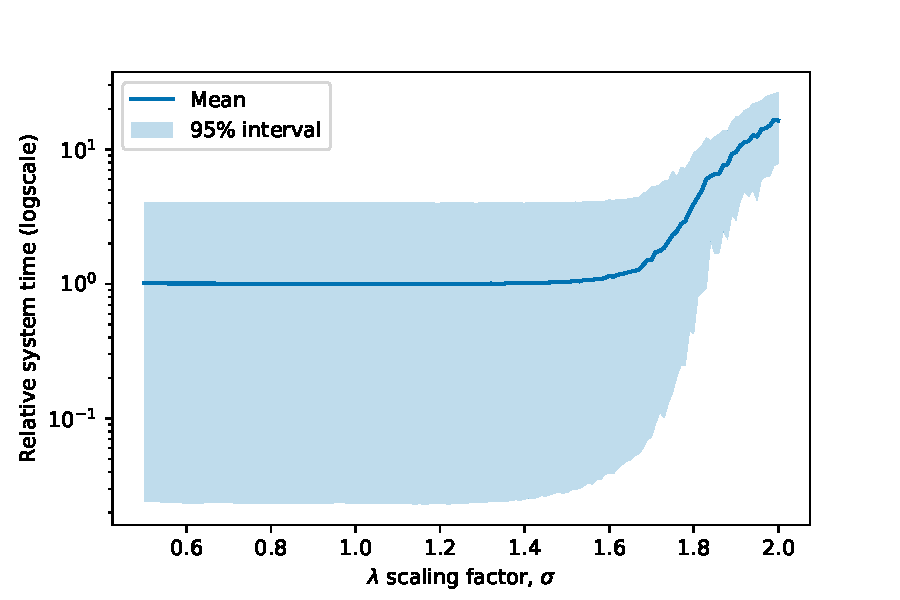
\includegraphics[width=\linewidth]{lambda_time}
        \caption{}\label{fig:lambda_time}
    \end{subfigure}\hfill%
    \begin{subfigure}{.5\imgwidth}
        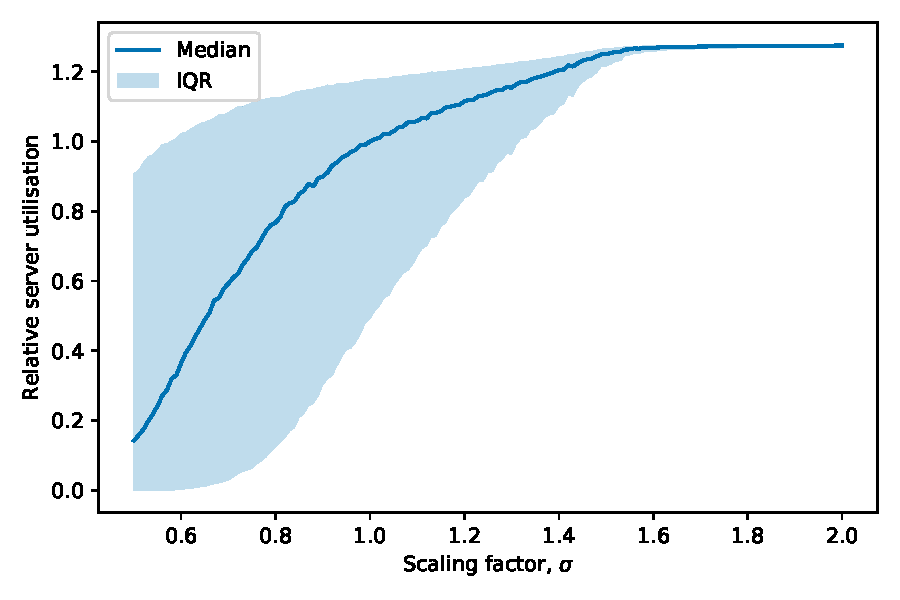
\includegraphics[width=\linewidth]{lambda_util}
        \caption{}\label{fig:lambda_util}
    \end{subfigure}
    \caption{%
        Plots of \(\sigma\) against relative (\subref{fig:lambda_time})~system
        time and (\subref{fig:lambda_util})~server utilisation.
    }\label{fig:lambda}
\end{figure}

Figure~\ref{fig:lambda} shows the effects of changing patient arrivals on
(\subref{fig:lambda_time})~relative system times and
(\subref{fig:lambda_util})~relative server utilisation over values of \(\sigma\)
from 0.5% to 2.0% at a
precision of \(1.0 \times 10^{-2}\)%. Specifically, each plot in the
figure (and the subsequent figures in this section) shows the median and
interquartile range (IQR) of each relative attribute. These metrics provide an
insight into the experience of the average user (or server) in the system, and
in the stability or variation of the body of users (servers).

What is evident from these plots is that things are happening as one might
expect: as arrivals increase, the strain on the system increases. However, it
should be noted that it also appears that the model has some amount of slack
relative to the base case. Looking at Figure~\ref{fig:lambda_time}, for
instance, the relative system times (i.e.\ the relative length of stay for
patients) remains unchanged up to \(\sigma \approx 1.2\), or an approximate 20\%
increase in arrivals of COPD patients. Beyond that, relative system times rise
to an untenable point where the median time becomes orders of magnitude above
the norm.

However, Figure~\ref{fig:lambda_util} shows that the situation for the system's
resources reaches its worst case near to the start of that spike in relative
system times (at \(\sigma \approx 1.4\)). That is, the median server utilisation
reaches a maximum (this corresponds to constant utilisation) at this point and
the variation in server utilisation disappears entirely.


\subsection{Changes to resource availability}\label{subsec:resources}

As is discussed in Section~\ref{sec:model}, the resource availability of the
system is captured by the number of parallel servers in the system, \(c\).
Therefore, to modify the overall resource availability, only the number of
servers need be changed. This kind of sensitivity analysis is usually done to
determine the opportunity cost of adding service capacity to a system, e.g.\
would adding \(n\) servers sufficiently increase efficiency without exceeding
a budget?

To reiterate the beginning of this section, all suitable parameters are given in
relative terms. This includes the number of servers here. By doing this, the
changes in resource availability are more easily seen, and do away with any
concerns as to what a particular number of servers exactly reflects in the real
world.

\begin{figure}
    \centering
    \begin{subfigure}{.5\imgwidth}
        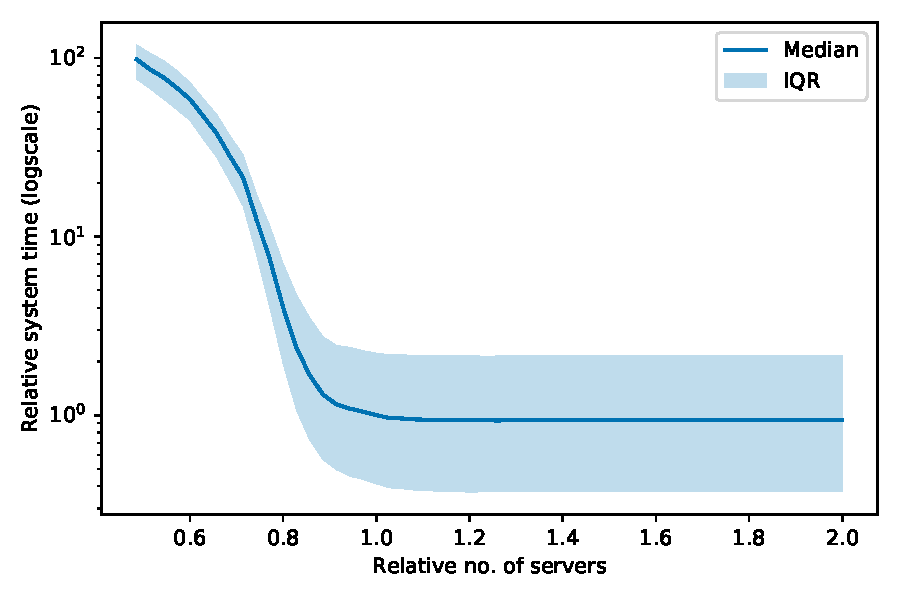
\includegraphics[width=\linewidth]{servers_time}
        \caption{}\label{fig:servers_time}
    \end{subfigure}\hfill%
    \begin{subfigure}{.5\imgwidth}
        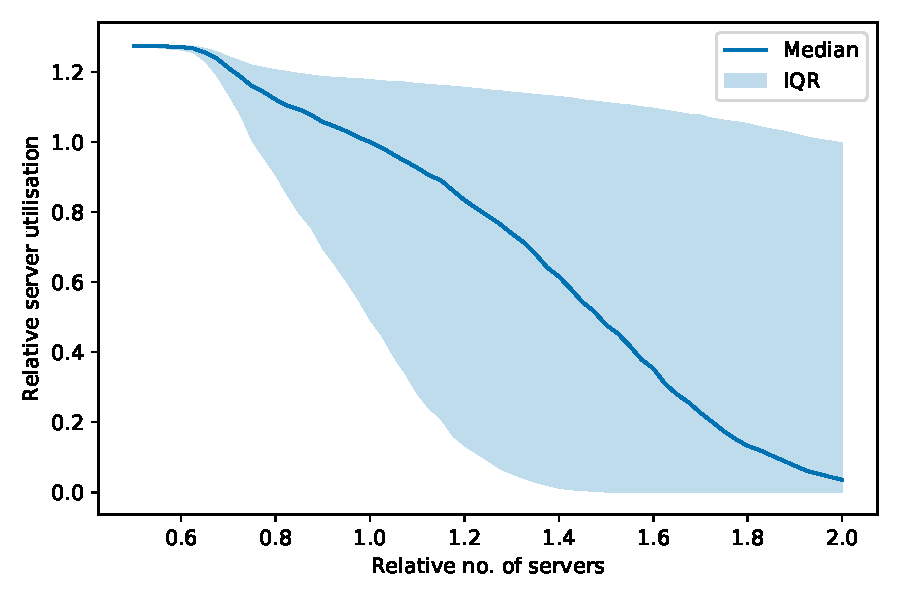
\includegraphics[width=\linewidth]{servers_util}
        \caption{}\label{fig:servers_util}
    \end{subfigure}
    \caption{%
        Plots of the relative number of servers against relative
        (\subref{fig:servers_time})~system time and
        (\subref{fig:servers_util})~server utilisation.
    }\label{fig:servers}
\end{figure}

Figure~\ref{fig:servers} shows how the relative resource availability affects
relative system times and server utilisation. In this scenario, the relative
number of servers took values from 0.5% to
2.0% at steps of
\(2.9 \times 10^{-2}\)% --- this is equivalent to a step size of 1
in the actual number of servers. Overall, these figures fortify the
claim from the previous scenario that there is some room to manoeuvre so that
the system runs `as normal' but pressing on those boundaries results in massive
changes to both resource requirements and system times.

In Figure~\ref{fig:servers_time} this amounts to a maximum of 20\% slack in
resources before relative system times are affected; further reductions quickly
result in a potentially tenfold increase in the median system time, and up to 50
times once resource availability falls by 50\%. Moreover, the variation in the
body of the relative times (i.e.\ the IQR) decreases as resource availability
decreases. The reality of this is that patients arriving at a hospital are
forced to consume larger amounts of resources (simply by being in a hospital)
regardless of their condition, putting added strains on the system.

Meanwhile, it appears that there is no tangible change in relative system times
given an increase in the number of servers. This indicates that the model
carries sufficient resources to cater to the population under normal
circumstances, and that adding service capacity will not necessarily improve
system times.

Again, Figure~\ref{fig:servers_util} shows that there is a substantial change in
the variation in the relative utilisation of the servers. In this case, the
variation dissipates as resource levels fall and increases as they increase.
While the relationship between real hospital resources and the number of servers
is not exact, having variation in server utilisation would suggest that parts of
the system may be configured or partitioned away in the case of some significant
public health event (such as a global pandemic) without overloading the system.


\subsection{Moving arrivals between clusters}\label{subsec:moving}

This scenario is perhaps the most relevant to actionable public health research
of those presented here. The clusters identified in this work could be
characterised by their clinical complexities and resource requirements, as done
in Section~\ref{subsec:overview}. Therefore, being able to model the movement of
some proportion of patient spells from one cluster to another will reveal how
those complexities and requirements affect the system itself. The reality is
then that if some public health policy could be implemented to enact that
movement informed by a model such as this then real change would be seen in the
real system.

In order to model the effects of spells moving between two clusters, the
assumption is that services remain the same (and so does each cluster's \(p_i\))
but their arrival rates are altered according to some transfer proportion.
Consider two clusters indexed at \(i, j\), and their respective arrival rates,
\(\lambda_i, \lambda_j\), and let \(\delta \in [0, 1]\) denote the proportion of
arrivals to be moved from cluster \(i\) to cluster \(j\). Then the new arrival
rates for each cluster, denoted by \(\hat\lambda_i, \hat\lambda_j\)
respectively, are:
\begin{equation}\label{eq:moving}
    \hat\lambda_i = \left(1 - \delta\right) \lambda_i
    \quad \text{and} \quad
    \hat\lambda_j = \delta\lambda_i + \lambda_j
\end{equation}

By moving patient arrivals between clusters in this way, the overall arrivals
are left the same since the sum of the arrival rates is the same. Hence, the
(relative) effect on server utilisation and system time can be measured
independently.

Figures~\ref{fig:moving_time}~and~\ref{fig:moving_util} show the effect of
moving patient arrivals between clusters on relative system time and relative
server utilisation respectively. In each figure, the median and IQR for the
corresponding attribute is shown, as in the previous scenarios. Each scenario
was simulated using values of \(\delta\) from 0.0% to
1.0% at steps of \(1.0 \times 10^{-1}\)%.

Considering Figure~\ref{fig:moving_time}, it is clear that there are some cases
where reducing particular types of spells (by making them like another type of
spell) has no effect on overall system times. Namely, moving the high
resource requirement spells that make up Cluster 0 and Cluster 3 to any other
cluster. These clusters make up only 10\% of all arrivals and this figure shows
that in terms of system times the model is able to handle them without concern
under normal conditions. The concern comes when either of the other clusters
moves to Cluster 0 or Cluster 3. Even as few as one in five of the low
complexity, low resource needs arrivals in Cluster 2 moving to either cluster
results in large jumps in the median system time for all arrivals, and soon
after, as in the previous scenario, any variation in the system times
disappears indicating an overborne system.

With relative server utilisation, the story is much the same. The normal levels
of high complexity, high resource arrivals from Cluster 3 are absorbed by the
system and moving these arrivals to another cluster bears no effect on resource
consumption levels. Likewise, either of the low resource need clusters moving
even slightly toward high resource requirements completely overruns the system's
resources. However, the relative utilisation levels of the system resources can
be reduced by moving arrivals from Cluster 0 to either Cluster 1 or Cluster 2,
i.e.\ by reducing the overall resource requirements of such spells.

In essence, this entire analysis offers two messages: that there are several
ways in which the system can get worse and even overwhelmed but, more
importantly, that any meaningful impact on the system must come from a stimulus
outside of the system that results in more healthy patients arriving to the
hospital. This is non-trivial; the first two scenarios in this analysis show
that there are no quick solutions to reduce the effect of COPD patients on
hospital capacity or length of stay. The only effective intervention is found
through inter-cluster transfers.

\begin{figure}
    \centering
    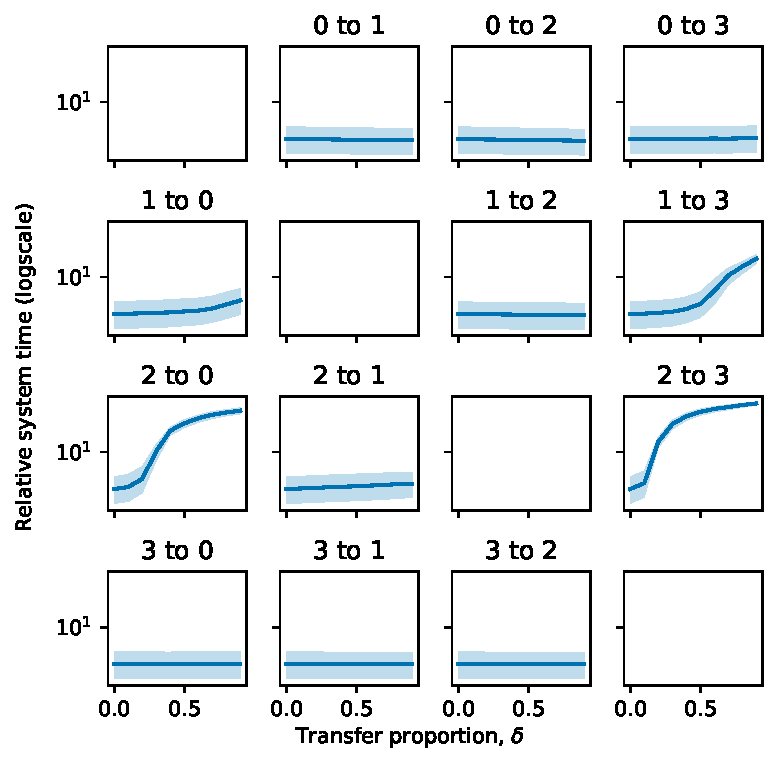
\includegraphics[width=\imgwidth]{moving_time}
    \caption{%
        Plots of proportions of each cluster moving to another against relative
        system time.
    }\label{fig:moving_time}
\end{figure}

\begin{figure}
    \centering
    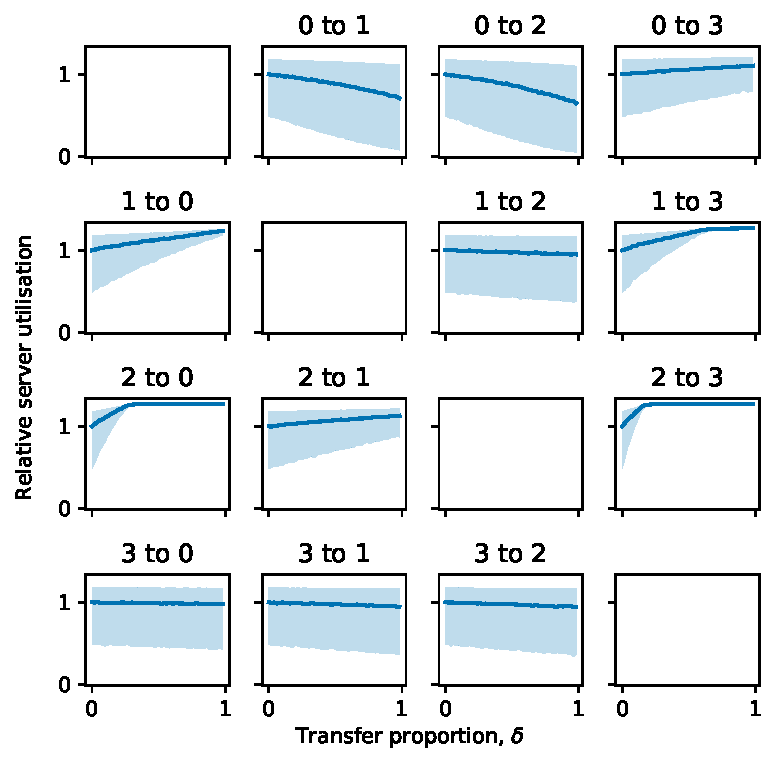
\includegraphics[width=\imgwidth]{moving_util}
    \caption{%
        Plots of proportions of each cluster moving to another on relative
        server utilisation.
    }\label{fig:moving_util}
\end{figure}
